\chapter{\IfLanguageName{dutch}{Stand van zaken}{State of the art}}%
\label{ch:stand-van-zaken}

% Tip: Begin elk hoofdstuk met een paragraaf inleiding die beschrijft hoe
% dit hoofdstuk past binnen het geheel van de bachelorproef. Geef in het
% bijzonder aan wat de link is met het vorige en volgende hoofdstuk.

% Pas na deze inleidende paragraaf komt de eerste sectiehoofding.

\section{\IfLanguageName{dutch}{Wat is een database?}{What is a database?}}%
\label{sec:wat-is-een-database}

Een database is de naam gegeven aan een elektronisch systeem dat zorgt voor het verzamelen, organiseren en linken van gegevens.~\autocite{ICTInformatiecentrum} Een voorbeeld hiervan is een mode winkel die gebruik maakt van een database om alle gegevens bij te houden die belangrijk zijn voor haar activiteit. Denk bijvoorbeeld aan gegevens over de producten die te koop zijn, gegevens over de klanten, gegevens over de bestellingen, enzovoort. Er bestaan echter verschillende soorten databases, elk met hun eigen set aan voor- en nadelen. Bovendien is niet elke database even schaalbaar. Sommige databases schalen beter verticaal dan horizontaal terwijl dit bij andere net het tegenovergestelde is. Nog andere kunnen dan weer schalen in beide richtingen.

\section{\IfLanguageName{dutch}{Schaalbaarheid}{Scalibility}}%
\label{sec:schaalbaarheid}

Hoewel een systeem vandaag betrouwbaar werkt, kan niet verzekerd worden dat dit zelfde systeem even betrouwbaar zal blijven werken in de toekomst. Volgens~\textcite{Kleppmann2017a} zou een veel voorkomende reden van de achteruitgang van databasesystemen liggen aan de toenemende belasting. Een systeem kan bijvoorbeeld origineel gebouwd zijn om een 10.000 tal gebruikers gelijktijdig te ondersteunen, het kan echter zijn dat het platform stijgt van 10 naar 100.000 gebruikers tegelijkertijd. Dit zorgt ervoor dat het systeem veel meer gegevens zal moeten kunnen verwerken dan voorheen.

Schaalbaarheid staat voor de mate waarin in dit geval een database systeem, haar capaciteit kan opvoeren indien de huidige omstandigheden niet meer voldoen aan de vraag uit de markt.~\autocite{Encyclo.nl} Schaalbaarheid is met andere woorden een term die gebruikt wordt om het vermogen van een systeem om om te gaan met een toenemende belasting te beschrijven.

Een database voldoet niet meer aan de vereisten wanneer deze bijvoorbeeld te traag wordt, niet meer efficiënt is, of andere prestatieproblemen vertoont. Naast prestatieproblemen zijn er nog andere situaties waarin een database niet meer aan de vereisten voldoet. Zoals bijvoorbeeld wanneer de database zijn opslagruimte ontoereikend wordt en de groei van gegevens niet meer kan accommoderen, de beveiliging van de database niet meer optimaal is, gebrek aan ondersteuning voor nieuwe technologieën enzovoort.

\subsection{\IfLanguageName{dutch}{Belasting}{Workload}}%
\label{subsec:workload}

De belasting op een database verwijst in deze context naar de hoeveelheid 'werk' die een database moet kunnen verwerken. Neem bijvoorbeeld een online winkel of een e-commerce webshop in de mode-industrie. Op deze website bekijken duizenden mensen dagelijks tegelijkertijd de verschillende producten die te koop zijn, voegen items toe aan hun winkelmandje, rekenen hun bestelling af en veel meer. Elk van deze acties genereert een verzoek naar de database, zoals het ophalen van productinformatie, bijwerken van voorraadgegevens, verwerken van betalingen enzovoort. Dit cumulatieve werk dat de database moet verrichten, wordt belasting genoemd.

Wanneer de belasting op een database die niet goed is opgesteld toeneemt, kan dit echter voor onvoorziene problemen zorgen. Het kan voorkomen dat een database niet snel genoeg kan antwoorden op alle verzoeken die binnenkomen. Hierdoor kan de website vertragen wat vertaalt kan worden in een minder goede gebruikerservaring. De schaalbaarheid van een database speelt hier een belangrijke rol om dergelijke problemen tegen te gaan en/of op te lossen.


\subsection{\IfLanguageName{dutch}{Horizontale en verticale schaalbaarheid}{Horizontal and vertical scaling}}%
\label{subsec:horizontale-en-verticale-schaalbaarheid}

In de context van databases kan de schaalbaarheid onderverdeeld worden in twee verschillende categorieën. Horizontale schaalbaarheid (het uitbreiden van een systeem op één machine over meerdere kleinere machines) en verticale schaalbaarheid (opwaarts schalen, van de huidige machine naar krachtigere machines gaan), zoals geïllustreerd in figuur~\ref{fig:scalability}. 

\begin{figure}[H]
    \centering
    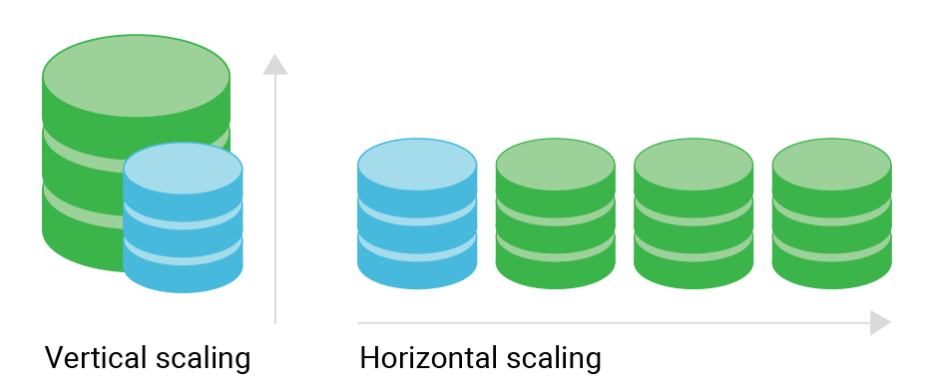
\includegraphics[width=\linewidth]{ScalabilityDiagram.png}
    \caption[Horizontale vs Verticale schaling]{Horizontale vs Verticale schaling ~\autocite{ScyllaDB}}
    \label{fig:scalability}
\end{figure}

Het draaien van een database op één enkele machine is vaak veel simpeler, dan de belasting verdelen over meerdere kleine machines.

Dit komt omdat het overstappen van een enkele node naar een gedistribueerde opstelling voor data met state veel extra complexiteit met zich mee kan brengen. Lange tijd werd het advies gegeven om de database op één enkele node te houden (op te schalen). Door de toename van de kosten van opschalen en de behoefte aan hoge beschikbaarheid ontstond de noodzaak om het systeem gedistribueerd te maken. Doordat krachtige machines extreem duur kunnen worden is het dus soms niet anders mogelijk dan horizontaal te schalen.~\autocite{Kleppmann2017} 

\section{\IfLanguageName{dutch}{Soorten databases}{Types of databases}}%
\label{sec:soorten-databases}

Er bestaan reeds verschillende soorten systemen om databases in te richten en voortdurend worden er nog nieuwe systemen bedacht.~\autocite{ictportal2022} Enkele van de meest voorkomende systemen zijn:
\begin{itemize}
      \item Flat file databases
      \item Relationele databases
      \item Gedistribueerde databases
      \item NoSQL databases
      \item Object georiënteerde databases
\end{itemize}

\newpage

\section{\IfLanguageName{dutch}{Flat file databases}{Flat file databases}}%
\emergencystretch 3em
\label{sec:flat-file-database}

Een flat file database wordt beschouwd als één van de eenvoudigste database systemen. Dit systeem omvat het opslaan van gegevens in een binair document of plain tekst document zoals CSV, txt, of TSV. Een flat file database heeft slechts een entry per regel. Bij deze database worden records van elkaar gescheiden door gebruik te maken van scheidingstekens zoals tabs en komma's. Volgens ~\textcite{geeksforgeeks2024} heeft een flat file database als voordeel dat het eenvoudig te assimileren is en efficiënt is bij het sorteren van de resultaten. Zoals elke soort database heeft de flat file database zijn voor- en nadelen. Enerzijds biedt de flat file database veel flexibiliteit en is het door zijn manier van dataopslag ook gemakkelijker voor mensen om de data te lezen. Daarnaast is deze database gebruiksvriendelijk en kan ze de snelheid van het testen en ontwikkelen verhogen. Anderzijds, doordat de flat file database slechts één tabel heeft, bestaat het gevaar van data redundantie. Bovendien biedt een flat file database beperkte functionaliteiten en is de beveiliging ook zwakker. Het beheren van een flat file database kan ook duur worden, zeker voor grote applicaties.

\section{\IfLanguageName{dutch}{Relationele databases}{Relational databases}}%
\label{sec:relationele-databases}

Een ander type database is de relationele database. Dit soort database zorgt voor het opslaan van gegevens in verschillende tabellen, waarbij elke tabel zijn gegevens organiseert in rijen en kolommen. Elke rij in een tabel stelt een record voor. Elke kolom staat voor een attribuut (bv. Naam of E-mail). Door gebruik te maken van unieke primaire of vreemde sleutels kunnen tabellen ook gelinkt worden aan elkaar. Deze identificateurs tonen de verschillende relaties die bestaan tussen de tabellen.~\autocite{ibm} Enkele voorbeelden van relationele databases zijn:  MariaDB, MySQL, PostgreSQL, enzovoort. Het grootste voordeel van een relationele database is de mogelijkheid voor het toevoegen van relaties tussen verschillende tabellen. Daarnaast is een relationele database ook redelijk makkelijk in gebruik, biedt het een verminderde redundantie en is het makkelijk om een back-up te nemen in geval van bijvoorbeeld een ramp.  Aan de andere kant kunnen niet alle gegevens worden opgeslagen in tabellen. Ongestructureerde of abstracte gegevens (zoals bijvoorbeeld afbeeldingen) zijn minder geschikt voor een relationele database. Maar ook de onmogelijkheid om gegevens hiërarchisch te rangschikken en de gegevenssegmentatie zijn enkele negatieve punten van een relationele database. ~\autocite{ovhcloud} Een relationele database hangt sterk samen met een object georiënteerde database. Voor het opstellen van een database van deze soort is het bijvoorbeeld mogelijk om gebruik te maken van een Entity Relational model (ER-model). Dit wordt geïllustreerd in figuur~\ref{fig:erd}.
 Het ER-model is ontworpen voor het identificeren van entiteiten en hun onderlinge relaties. Op basis van dit model kan een schema opgesteld worden die de logische structuren van een database grafisch kan weergeven. ~\autocite{lucidchart}
 \begin{figure}[H]
     \centering
     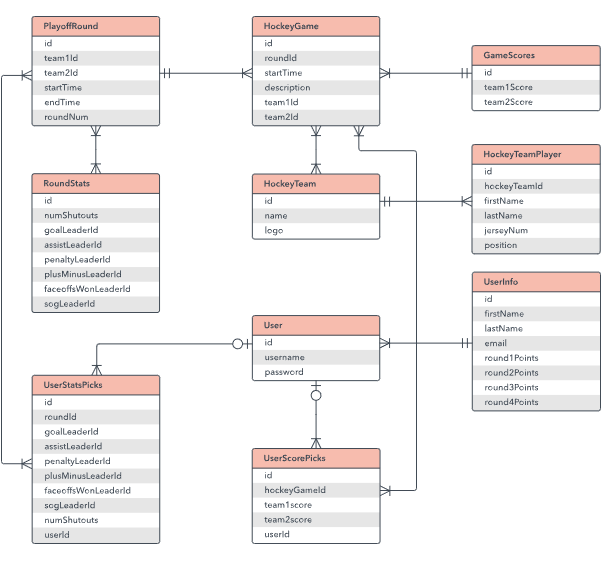
\includegraphics[width=\linewidth]{erd.png}
     \caption[Entity Relationship Diagram (ERD)]{Entity Relationship Diagram (ERD) ~\autocite{lucidchart}}
     \label{fig:erd}
 \end{figure}



\section{\IfLanguageName{dutch}{Gedistribueerde databases}{Distributed databases}}%
\label{sec:gedistribueerde-databases}

Een gedistribueerd database systeem is technisch gezien een database die niet gelimiteerd is tot één systeem. Volgens ~\textcite{DistributedDatabase2022} is het een soort van database systeem dat bestaat uit een groep van computers die onderling met elkaar verbonden zijn en die het doen lijken alsof het één enkel systeem is. Op deze manier kan de database toegankelijk gemaakt worden voor verschillende gebruikers over de hele wereld. Het is echter belangrijk dat de database zo beheerd wordt dat het voor de gebruikers lijkt alsof er slechts één enkele database is. 

Er zijn twee soorten gedistribueerde databases. Homogene databases en heterogene databases.


\begin{itemize}
      \item \textbf{\textit{Homogene databases}} \\
            Zoals de naam suggereert, slaan alle verschillende sites de database op een identieke manier op. Niet enkel de gegevens maar ook het besturingssysteem, het databasebeheersysteem en de gebruikte datastructuren zijn allemaal hetzelfde op alle locaties. Deze manier van werken maakt het makkelijk om te beheren.

      \item \textbf{\textit{Heterogene databases}} \\
            Bij heterogene databases kunnen de sites verschillende schema’s en software gebruiken wat uiteindelijk kan leiden tot problemen bij bijvoorbeeld de verwerking van zoekopdrachten. Bij dit soort database is het belangrijk dat er vertalingen plaatsvinden om het mogelijk te maken om verschillende sites met elkaar te doen communiceren.
\end{itemize}

Door het gebruik van meerdere sites heeft een gedistribueerde database een snelle gegevensverwerking. Het systeem is het meest van de tijd online. Hierdoor is de betrouwbaarheid en beschikbaarheid hoog. Het gebruik van verschillende sites maakt het ook makkelijk om de database uit te breiden. Gedistribueerde database systemen hebben daarbovenop ook een relatief lage bedrijfskost. Het beheren van dergelijk systeem kan echter heel complex worden, vooral wat betreft de beveiligingsproblemen.

\section{\IfLanguageName{dutch}{NoSQL databases}{NoSQL databases}}%
\emergencystretch 3em
\label{sec:NoSQL-databases}

Een “not only SQL” database of “non-SQL” database, kortweg ook wel NoSQL database genoemd, is een type database die ontworpen is om grote hoeveelheden aan ongestructureerde of half gestructureerde data op te slaan en te verwerken op andere manieren dan een relationele database dat doet met rijen en tabellen.~\autocite{DistributedDatabase2022} Er zijn verschillende soorten NoSQL databases. De vier meest voorkomende zijn:

\begin{itemize}
      \item \textbf{\textit{Sleutel-waarde paren}} \\
            Bij deze soort database worden gegevens opgeslagen in de vorm van sleutel-waarde paren met behulp van een hashtabel.~\autocite{Microsoft} 
            Voor elke sleutel, die opgeslagen wordt als een string, hoort een waarde die opgeslagen kan worden als String, JSON, XML, etc. Doordat dit type database heel simplistisch is en makkelijk in gebruik, is de response tijd ook enorm snel. Daarnaast is het ook mogelijk om deze database zowel verticaal als horizontaal te schalen. Door de simpliciteit van de database is het echter niet mogelijk om queries, zoekopdrachten op een database, over te dragen van een database naar de andere, wat kan helpen bij het optimaliseren van prestaties, flexibiliteit en de schaalbaarheid. Daarnaast is de sleutel-waarde store niet geoptimaliseerd voor complexe querybewerkingen, wat betekent dat de database niet kan worden bevraagd zonder een specifieke sleutel. Enkele voorbeelden van de meest populaire sleutel-waarde paren database zijn bijvoorbeeld: Dynamo DB, Redis, BerkleyDB enzovoort.~\autocite{DistributedDatabase2022} Figuur~\ref{fig:keyvaluepair} is een voorbeeld van een sleutel-waarde database.
            \begin{figure}[H]
                \centering
                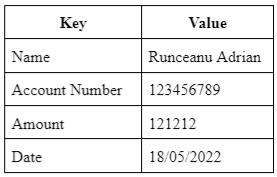
\includegraphics[width=0.3\textwidth]{keyvaluepair.png}
                \caption[Voorbeeld van een tabel die key-value paren bevat]{Voorbeeld van een tabel die key-value paren bevat ~\autocite{DistributedDatabase2022}}\label{fig:keyvaluepair}
            \end{figure}
            
      \item \textbf{\textit{Document}} \\
            Een document database vormt een uitbreiding op de sleutel-waarde paren door hele documenten te ordenen in groepen. Deze groepen worden verzamelingen genoemd.~\autocite{Microsoft} Door het schemaloze gedrag van een documentdatabase is dit soort database perfect uitgerust voor het behouden van de bestaande gegevens bij enorme volumes aan data. Bovendien is deze database zeer makkelijk te onderhouden, heeft het een heel eenvoudig bouwproces en bevat het ingebouwde versiebeheer. Naarmate de hoeveelheden data in de documenten groter worden, neemt de kans toe dat deze databases complexer worden. Versiebeheer zorgt er dan voor dat er minder conflicten ontstaan. Aan de andere kant heeft een documentdatabase ook enkele nadelen. Zo beschikt de database over een zwakke atomiciteit. Atomiciteit staat voor de A in de ACID-transacties \mbox{-} Atomicity, Consistency, Isolation en Durability. Dit betekent dat verschillende operaties gegroepeerd kunnen worden in een enkele entiteit.~\autocite{Oracle} Dit is echter niet van toepassing bij een document database. Daarnaast is de beveiliging van een document database ook niet optimaal. Door het ontbreken van ingebouwde mechanismen voor sterke authenticatie en autorisatie, kunnen gegevens kwetsbaar zijn voor ongeautoriseerde toegang. Enkele voorbeelden van een documentdatabase zijn: MongoDB, CouchDB, Amazon DocumentDB, Lotus Notes, enzovoort.~\autocite{DistributedDatabase2022} Figuur~\ref{fig:document} is een voorbeeld van een document database.
            
            \begin{figure}[H]
                \centering
                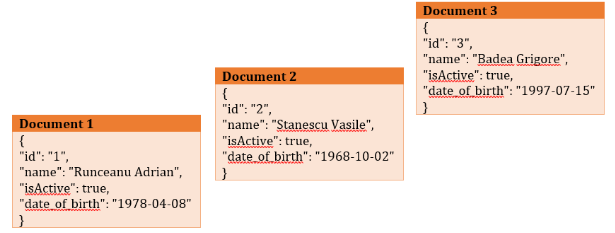
\includegraphics[width=0.7\linewidth]{graphics/document}
                \caption[Voorbeeld van een document database met key-value paren]{Voorbeeld van een document database met key-value paren ~\autocite{DistributedDatabase2022}}
                \label{fig:document}
            \end{figure}
            
      \item \textbf{\textit{Kolommen}} \\
            Bij een kolom database worden, zoals de naam suggereert, de gegevens efficiënt opgeslagen in kolommen en worden query's uitgevoerd op rijen met verspreide gegevens.~\autocite{Microsoft} Kolom databases worden vooral gebruikt voor taken die gerelateerd zijn aan big data. Dit is mogelijk door de snelheid en efficiëntie waarmee deze database analytische query’s uitvoert. Volgens ~\textcite{DistributedDatabase2022} is de database ook zeer persistent van aard, wat betekent dat de gegevens die opgeslagen zijn duurzaam en bestendig zijn tegen stroomuitval of andere storingen, waardoor ze behouden blijven en beschikbaar zijn voor toekomstig gebruik. De database is ook gedistribueerd en biedt een hoge flexibiliteit. Dit laat toe om verschillende bewerkingen uit te voeren, zoals het berekenen van het gemiddelde (AVG) en het berekenen van een minimum en maximum waarde (MIN, MAX). Kolom databases zijn echter minder geschikt voor relationele data. Door de complexiteit van de queries die uitgevoerd worden in e-commerce webshops, transactionele ondersteuning en real-time updatevereisten, is deze soort database minder geschikt voor e-commerce. Enkele voorbeelden van een kolom database zijn Google's Bigtable, Cassandra, HBase, Azure Tables, enzovoort.~\autocite{DistributedDatabase2022} In figuur~\ref{fig:column} wordt een voorbeeld van een kolom database gegeven.
            \begin{figure}[H]
                \centering
                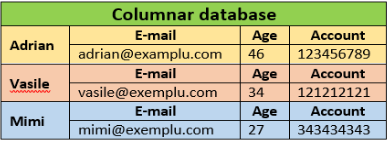
\includegraphics[width=0.7\linewidth]{graphics/column}
                \caption[Voorbeeld van een columnar database]{Voorbeeld van een columnar database ~\autocite{DistributedDatabase2022}}
                \label{fig:column}
            \end{figure}
            
      \item \textbf{\textit{Grafiek}} \\
            Bij grafiek databases wordt er gebruik gemaakt van knopen en edges om gegevens weer te geven die aan elkaar verbonden zijn. Knopen zijn de hoekpunten waarin gegevensobjecten worden opgeslagen. Tussen de verschillende knooppunten kunnen oneindig veel relaties bestaan. Deze relaties worden Edges genoemd.~\autocite{Amazon} Deze manier van werken zorgt ervoor dat er omgegaan kan worden met grote hoeveelheden aan data waarbij real-time query responses gedaan worden. Het nadeel aan deze database is echter dat het niet geschikt is voor elke type project. Grafiekdatabases zijn over het algemeen minder geschikt voor transactie intensieve toepassingen zoals e-commerce platforms. Een voorbeeld waarvoor dit type database dan wel weer zeer geschikt is, is fraudeopsporing. Een grafiekdatabase kan hier gebruikt worden voor het opsporen van de verdachte patronen en relaties tussen entiteiten.  Hoewel het mogelijk is om een grafiek database uit te breiden en te groeien is het eerder complex om deze database te schalen. Het is belangrijk dat alvorens een beslissing genomen wordt over het gebruik van deze database, de noden en de architectuur van het project vast staan. Enkele voorbeelden zijn: Neo4j, OrientDB, TypeDB, RedisGraph, TerminusDB, enzovoort.~\autocite{DistributedDatabase2022} Figuur~\ref{fig:grafiekdb} is een voorbeeld van een grafiek database.
            
            \begin{figure}[H]
                \centering
                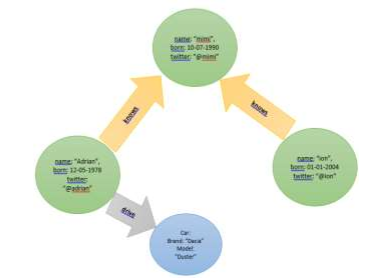
\includegraphics[width=0.7\linewidth]{graphics/grafiekdb}
                \caption[Voorbeeld grafiek database]{Voorbeeld grafiek database  ~\autocite{DistributedDatabase2022}}
                \label{fig:grafiekdb}
            \end{figure}
            
\end{itemize}

\section{\IfLanguageName{dutch}{Object georiënteerde databases (OOD)}{Object-oriented databases}}%
\label{sec:Object-georiënteerde-databases}

Een object georiënteerd database systeem is een systeem dat gebruik maakt van complexe dataobjecten. Deze dataobjecten zijn gebaseerd op de objecten die gebruikt worden in object georiënteerde programmeertalen zoals bijvoorbeeld Java, C++, enzovoort. In een object georiënteerde programmeertaal wordt alles bekeken vanuit het concept van “objecten” die zowel data (attributen) als procedures (methodes) kunnen bevatten. Een voorbeeld hiervan zou een kauwgomballenmachine kunnen zijn. Hierbij stellen de machine, de kauwgomballen en het muntstuk een object voor. Elk van deze objecten heeft eigenschappen die relevant zijn voor hun rol in het systeem en methodes die bepaalde acties mogelijk maken.~\autocite{MongoDB} Deze werkwijze verbetert de prestaties door minder vertaling tussen programmeertaal en database en verkort de ontwikkeltijd door directe interactie met database-objecten. Het ondersteunt complexe structuren en rijke datatypes, maar ondervindt moeilijkheden in adoptie, standaardisatie, kosten en integratie met andere systemen. De complexiteit van de implementatie en de benodigde expertise maken de adoptie ervan langzaam en kostbaar. Een voorbeeld van een OOD is MongoDB Realm.
\newpage
\section{\IfLanguageName{dutch}{Hoe zit het in de praktijk?}{What about in practice?}}%
\label{sec:De praktijk}

Wereldwijd zijn er een immens groot aantal e-commerce webshops waar de webshops in de mode-industrie een groot deel van uitmaken. Elk van deze webshops maakt gebruik van zijn eigen soort database. Het analyseren van elke webshop om de achterliggende database te achterhalen is een onbegonnen werk. Om deze reden wordt de stand van zaken gericht op de databases die gebruikt worden door het bedrijf van de co-promotor van deze bachelorproef, Aware. Binnen dit bedrijf wordt vooral gebruik gemaakt van MariaDB als database oplossing voor hun e-commerce vereisten, al dan niet binnen de mode-industrie. Aware maakt gebruik van MariaDB vanwege de schaalbaarheid en de brede acceptatie binnen de programmeurgemeenschap. Dit vergemakkelijkt de werving van nieuwe medewerkers, aangezien veel ontwikkelaars vertrouwd zijn met dit databaseplatform, wat resulteert in minder trainingsbehoeften. Bovendien staat MariaDB bekend om zijn snelheid, wat een belangrijke overweging was bij de keuze voor deze database. Echter, recentelijk werd er opgemerkt dat het ophalen van een groot aantal logs meer tijd in beslag neemt dan verwacht. Met name select queries, vooral deze met where clausules, ervaren aanzienlijke vertraging.